\documentclass{beamer}
\usetheme[pageofpages=of,% String used between the current page and the
                         % total page count.
          bullet=circle,% Use circles instead of squares for bullets.
          titleline=true,% Show a line below the frame title.
          alternativetitlepage=true,% Use the fancy title page.
	  titlepagelogo=logo-circl.pdf,% Logo for the first page.
%          watermark=watermark-polito,% Watermark used in every page.
%          watermarkheight=100px,% Height of the watermark.
%          watermarkheightmult=4,% The watermark image is 4 times bigger
                                % than watermarkheight.
          ]{Torino}

\usepackage[utf8x]{inputenc}
\usepackage{listings}
\usepackage{soul}
\usepackage{siunitx}
\usepackage{booktabs}
%\lstset{ 
%  backgroundcolor=\color{white},   % choose the background color; you must add \usepackage{color} or \usepackage{xcolor}
%  basicstyle=\footnotesize,        % the size of the fonts that are used for the code
%  breakatwhitespace=false
%}

\usepackage{tikz}
\usetikzlibrary{shapes,snakes,automata,positioning,matrix,fit}


\usepackage[listings]{tcolorbox}
\usepackage{xcolor}
\usepackage{colortbl}
\definecolor{mygreen}{rgb}{0,0.6,0}
\definecolor{mygreen2}{rgb}{0,0.56,0.16}
\definecolor{myred}{rgb}{0.6,0.066,0.066}
\definecolor{redCIRCL}{RGB}{213,43,30}
\definecolor{mygray}{rgb}{0.5,0.5,0.5}
\definecolor{mymauve}{rgb}{0.58,0,0.82}
\definecolor{mygray}{gray}{0.9}
\definecolor{mywhite}{rgb}{1,1,1}
\definecolor{myblack}{rgb}{0,0,0}
\definecolor{mybeige}{HTML}{eeeeee}
%\usepackage{tcolorbox}
\usepackage[listings]{tcolorbox}
\tcbuselibrary{listings}

\lstdefinestyle{code}{ %
  backgroundcolor=\color{mybeige},   % choose the background color; you must add \usepackage{color} or \usepackage{xcolor}; should come as last argument
  basicstyle=\footnotesize\ttfamily,        % the size of the fonts that are used for the code
  breakatwhitespace=false,         % sets if automatic breaks should only happen at whitespace
  breaklines=true,                 % sets automatic line breaking
  captionpos=b,                    % sets the caption-position to bottom
  commentstyle=\color{mygreen},    % comment style
  deletekeywords={...},            % if you want to delete keywords from the given language
  escapeinside={\%*}{*)},          % if you want to add LaTeX within your code
  extendedchars=true,              % lets you use non-ASCII characters; for 8-bits encodings only, does not work with UTF-8
  frame=single,	                   % adds a frame around the code
  keepspaces=true,                 % keeps spaces in text, useful for keeping indentation of code (possibly needs columns=flexible)
  keywordstyle=\color{blue},       % keyword style
  language=Python,                 % the language of the code
  morekeywords={*,...},           % if you want to add more keywords to the set
  numbers=left,                    % where to put the line-numbers; possible values are (none, left, right)
  numbersep=5pt,                   % how far the line-numbers are from the code
  numberstyle=\tiny\color{myblack}, % the style that is used for the line-numbers
  rulecolor=\color{black},         % if not set, the frame-color may be changed on line-breaks within not-black text (e.g. comments (green here))
  showspaces=false,                % show spaces everywhere adding particular underscores; it overrides 'showstringspaces'
  showstringspaces=false,          % underline spaces within strings only
  showtabs=false,                  % show tabs within strings adding particular underscores
  stepnumber=1,                    % the step between two line-numbers. If it's 1, each line will be numbered
  stringstyle=\color{mymauve},     % string literal style
  tabsize=2,	                   % sets default tabsize to 2 spaces
  title=\lstname                   % show the filename of files included with \lstinputlisting; also try caption instead of title
}
\lstdefinestyle{bash}{ %
  backgroundcolor=\color{black!85},   % choose the background color; you must add \usepackage{color} or \usepackage{xcolor}; should come as last argument
  basicstyle=\footnotesize\color{mywhite},        % the size of the fonts that are used for the code
  breakatwhitespace=false,         % sets if automatic breaks should only happen at whitespace
  breaklines=true,                 % sets automatic line breaking
  captionpos=b,                    % sets the caption-position to bottom
  commentstyle=\color{mygreen},    % comment style
  deletekeywords={...},            % if you want to delete keywords from the given language
  escapeinside={\%*}{*)},          % if you want to add LaTeX within your code
  extendedchars=true,              % lets you use non-ASCII characters; for 8-bits encodings only, does not work with UTF-8
  frame=single	                   % adds a frame around the code
  keepspaces=true,                 % keeps spaces in text, useful for keeping indentation of code (possibly needs columns=flexible)
  keywordstyle=\color{white}\bfseries,       % keyword style
  language=bash,                 % the language of the code
  morekeywords={*,$,git, clone,... },           % if you want to add more keywords to the set
  numbers=left,                    % where to put the line-numbers; possible values are (none, left, right)
  numbersep=5pt,                   % how far the line-numbers are from the code
  numberstyle=\tiny\color{mywhite}, % the style that is used for the line-numbers
  rulecolor=\color{black},         % if not set, the frame-color may be changed on line-breaks within not-black text (e.g. comments (green here))
  showspaces=false,                % show spaces everywhere adding particular underscores; it overrides 'showstringspaces'
  showstringspaces=false,          % underline spaces within strings only
  showtabs=false,                  % show tabs within strings adding particular underscores
  stepnumber=1,                    % the step between two line-numbers. If it's 1, each line will be numbered
  stringstyle=\color{mymauve},     % string literal style
  tabsize=2,	                   % sets default tabsize to 2 spaces
  title=\lstname                   % show the filename of files included with \lstinputlisting; also try caption instead of title
}
\lstdefinestyle{default}{ %
  backgroundcolor=\color{white},   % choose the background color; you must add \usepackage{color} or \usepackage{xcolor}; should come as last argument
  basicstyle=\footnotesize\color{black},        % the size of the fonts that are used for the code
  breakatwhitespace=false,         % sets if automatic breaks should only happen at whitespace
  breaklines=true,                 % sets automatic line breaking
  captionpos=b,                    % sets the caption-position to bottom
  commentstyle=\color{mygreen},    % comment style
  deletekeywords={...},            % if you want to delete keywords from the given language
  escapeinside={\%*}{*)},          % if you want to add LaTeX within your code
  extendedchars=true,              % lets you use non-ASCII characters; for 8-bits encodings only, does not work with UTF-8
  frame=single	                   % adds a frame around the code
  keepspaces=true,                 % keeps spaces in text, useful for keeping indentation of code (possibly needs columns=flexible)
  keywordstyle=\color{white}\bfseries,       % keyword style
  language=bash,                 % the language of the code
  morekeywords={*,$,git, clone,... },           % if you want to add more keywords to the set
  numbers=left,                    % where to put the line-numbers; possible values are (none, left, right)
  numbersep=5pt,                   % how far the line-numbers are from the code
  numberstyle=\tiny\color{black}, % the style that is used for the line-numbers
  rulecolor=\color{black},         % if not set, the frame-color may be changed on line-breaks within not-black text (e.g. comments (green here))
  showspaces=false,                % show spaces everywhere adding particular underscores; it overrides 'showstringspaces'
  showstringspaces=false,          % underline spaces within strings only
  showtabs=false,                  % show tabs within strings adding particular underscores
  stepnumber=1,                    % the step between two line-numbers. If it's 1, each line will be numbered
  stringstyle=\color{mymauve},     % string literal style
  tabsize=2,	                   % sets default tabsize to 2 spaces
  title=\lstname                   % show the filename of files included with \lstinputlisting; also try caption instead of title
}
\lstset{style=code}


\AtBeginSection[]{
  \begin{frame}
  \vfill
  \centering
  \begin{beamercolorbox}[sep=8pt,center,shadow=true,rounded=true]{title}
      {\color{white} \usebeamerfont{title}\insertsectionhead}\par%
  \end{beamercolorbox}
  \vfill
  \end{frame}
}

% all authors
%\author{\Large{Alexandre Dulaunoy}\\ \scriptsize{alexandre.dulaunoy@circl.lu}\\ \large{Aurelien Thirion}\\ \scriptsize{aurelien.thirion@circl.lu}\\ \large{Jean-Louis Huynen}\\ \scriptsize{jean-louis.huynen@circl.lu}\\ \Large{Sami Mokaddem}\\ \scriptsize{sami.mokaddem@circl.lu}}
% all presentation
\author{\large{Aurelien Thirion}\\ \scriptsize{aurelien.thirion@circl.lu}\\ \large{Gerard Wagener}\\ \scriptsize{gerard.wagener@circl.lu}}
\title{AIL Project}
\subtitle{Practical and Efficient Data-Mining of Chats, Suspicious Websites, Forums and Tor Hidden-Services}
\institute{info@circl.lu}
\date{\today}

\begin{document}


\begin{frame}[t,plain]
\titlepage
\end{frame}

\begin{frame}
   \frametitle{Background}
\begin{itemize}
    \item Over the past five years, we have developed the AIL project\footnote{\url{https://www.ail-project.org/}} to fulfill our needs at CIRCL in intelligence gathering and analysis.
    \item AIL features an extensible Python-based framework for the {\bf analysis of unstructured information}, collected either through an advanced Crawler manager or from various feeders, including social networks and custom feeders.
    \item The AIL Project is an {\bf open-source} framework\footnote{\url{https://github.com/ail-project}} comprising various modules designed for the {\bf collection, crawling, digging, and analysis of unstructured data}.
	\begin{figure}
        
\includegraphics[scale=0.1, angle=0]{images/ail-project.png}
    \end{figure}
\end{itemize}
\end{frame}

% collection issue

\begin{frame}
    \frametitle{High Level Overview}
    \begin{center}
        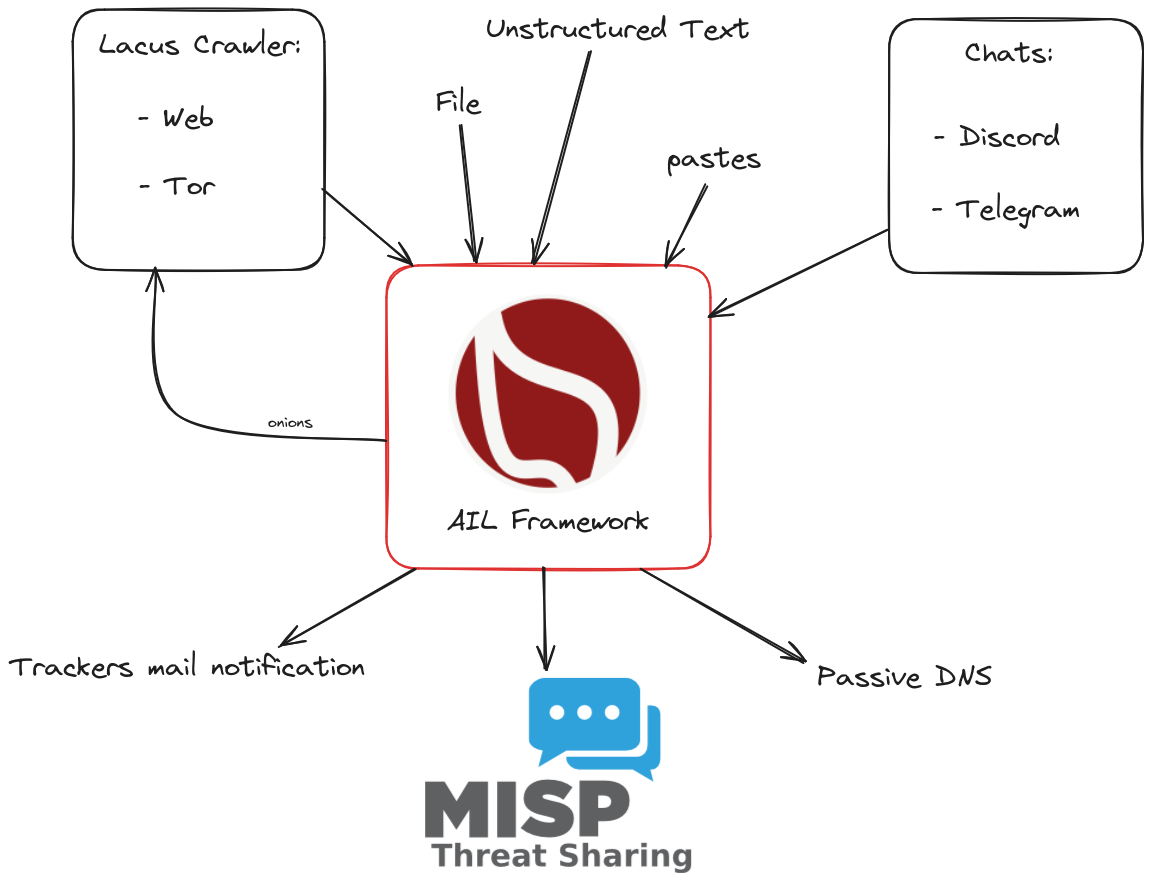
\includegraphics[scale=0.24]{images/ail-overview.png}
    \end{center}
\end{frame}

\begin{frame}
    \frametitle{{\it Collection} - automate crawling}

\begin{itemize}
    \item Crawling can be a challenging task, for example, gathering all the blog posts from ransomware groups\footnote{\url{https://www.ransomlook.io/}}, which can be demanding for an analyst.
    \item AIL offers a crawling feature that can {\bf initiate regular crawls using a standard spawned browser}.
\end{itemize}
    \begin{center}
        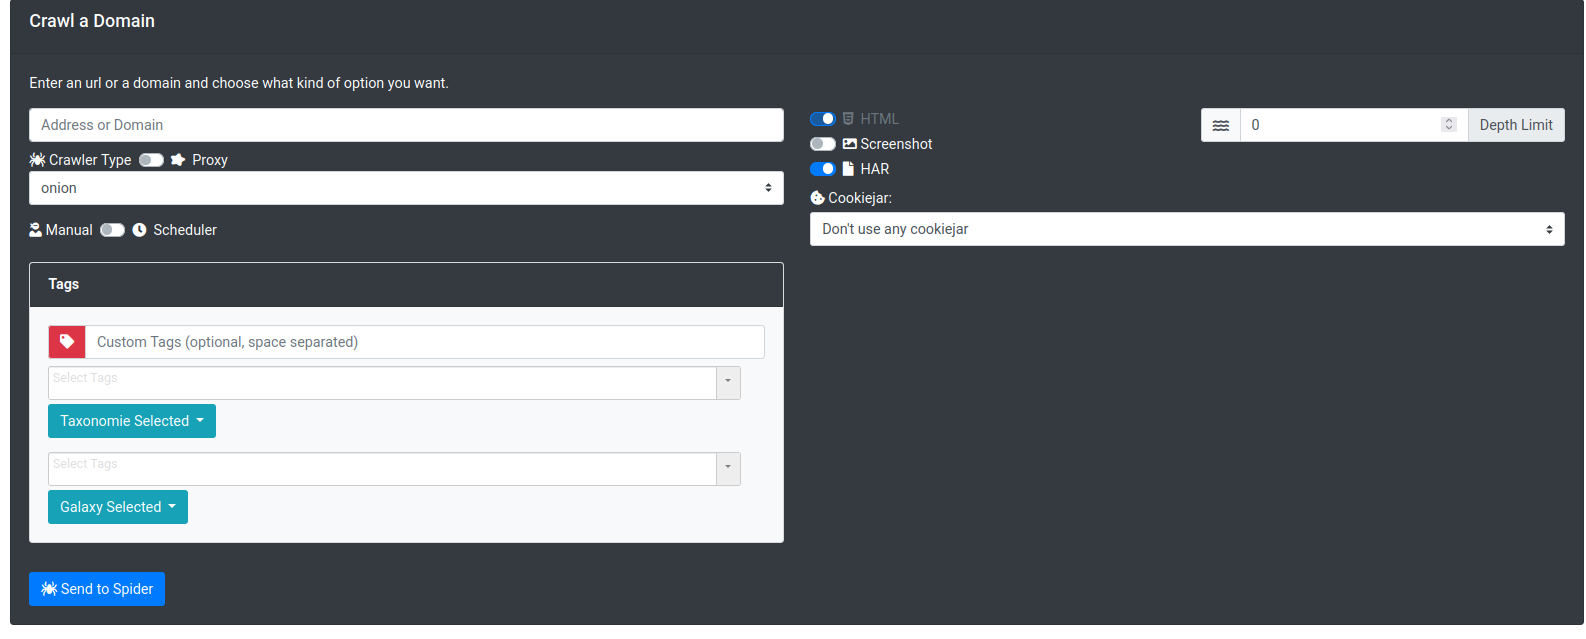
\includegraphics[scale=0.17]{images/ail-crawling.png}
    \end{center}
\end{frame}

% TODO deanonimize onions

\begin{frame}
    \frametitle{{\it Collection} - Lacus Crawler\footnote{\url{https://github.com/ail-project/lacus}}}
        	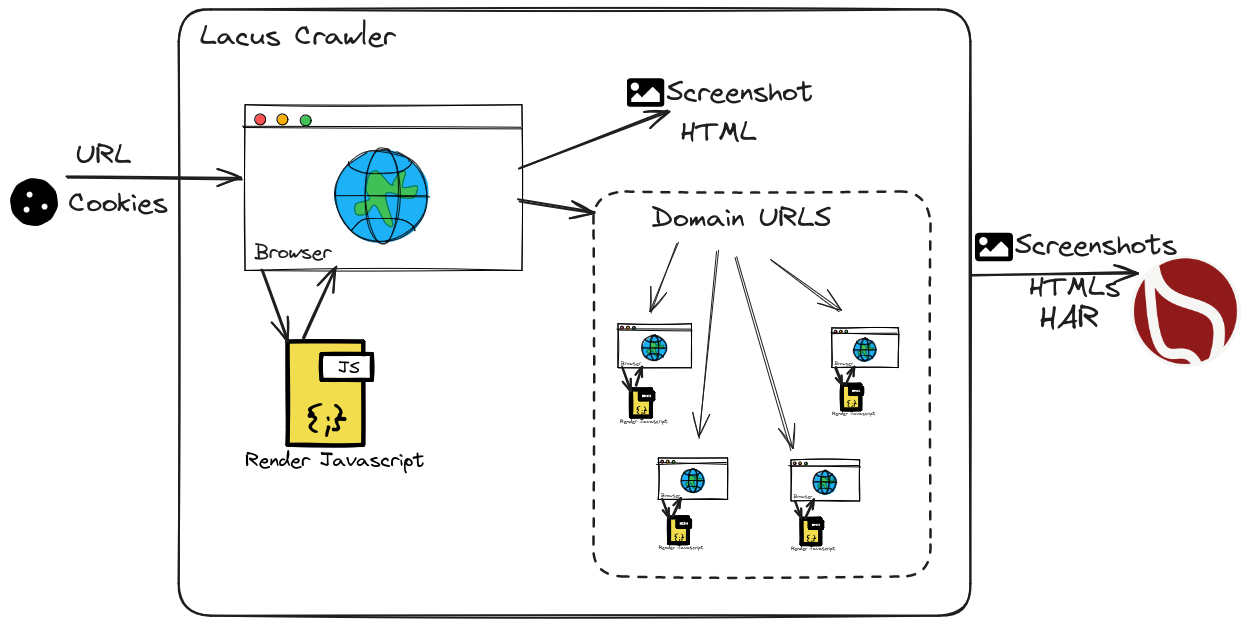
\includegraphics[scale=0.27]{images/ail-lacus.png}
\end{frame}


\begin{frame}
    \frametitle{Crawler: Cookiejar}
    Use your cookies to login and bypass captcha
    \centerline{
        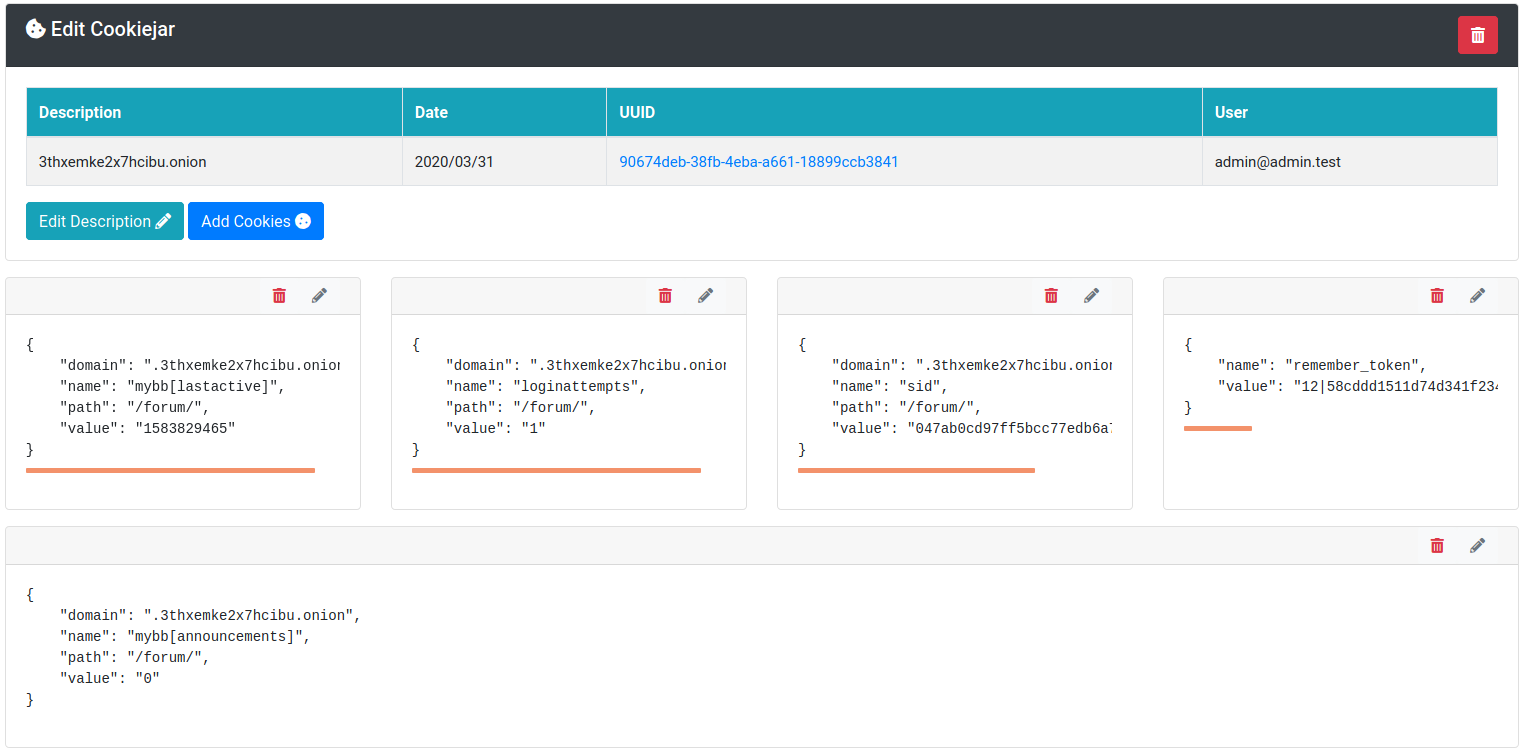
\includegraphics[scale=0.23]{screenshot/crawler-cookiejar-edit.png}
    }
\end{frame}

\begin{frame}
    \frametitle{Crawler: Cookiejar}
    \centerline{
        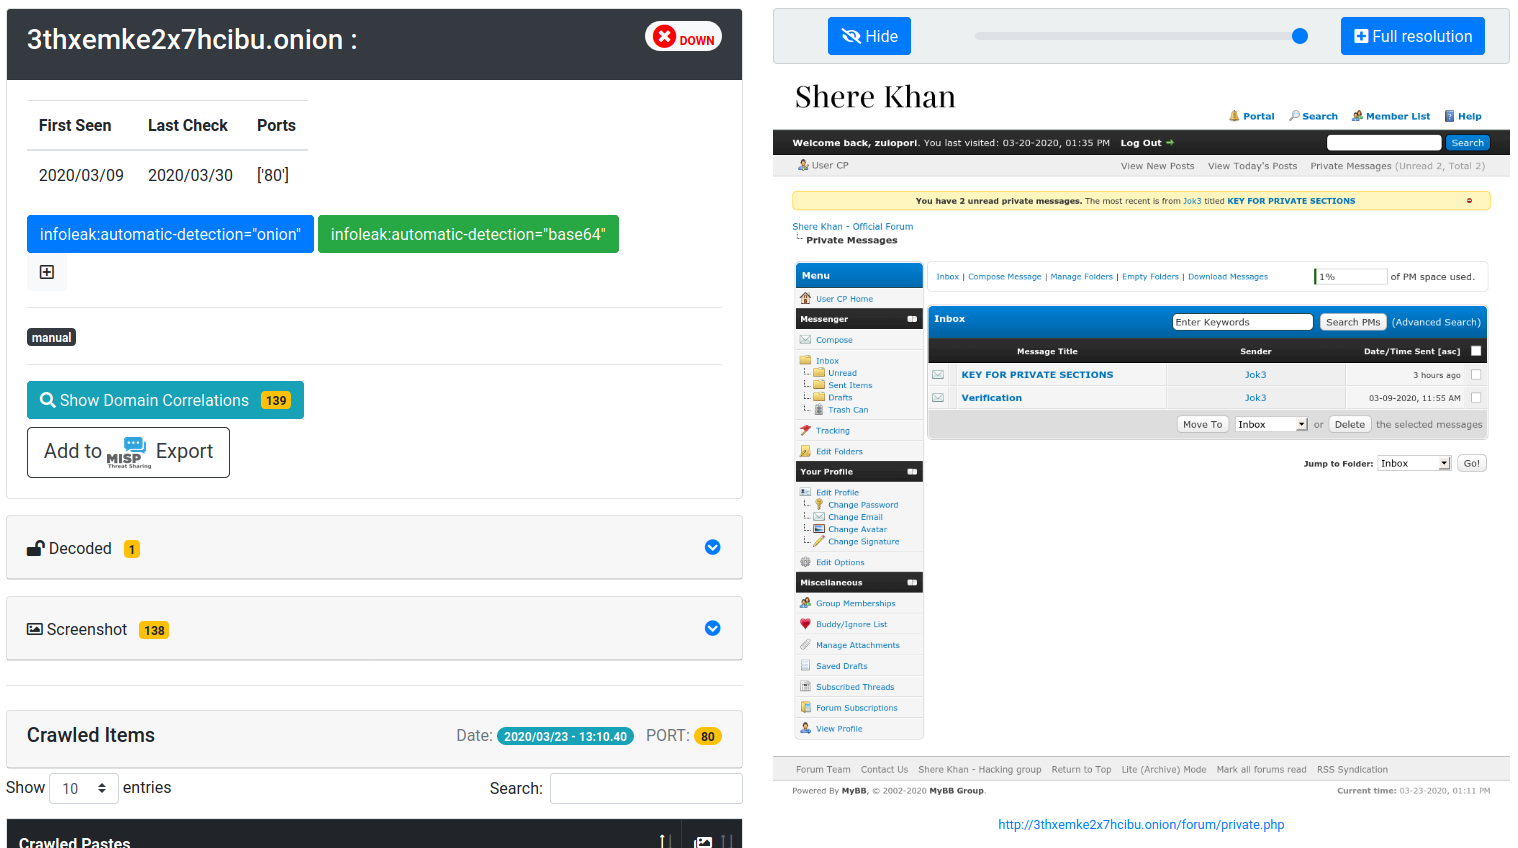
\includegraphics[scale=0.23]{screenshot/crawler-cookiejar-domain-crawled.png}
    }
\end{frame}


\begin{frame}
    \frametitle{{\it Collection} - automate collection}
	\begin{itemize}
		\item Collecting data from various chat sources can be a {\bf tedious task for analysts}.
		\item AIL offers a set of feeders (e.g., Telegram, Discord, etc.) that can be used to subscribe to chat channels.
        \item All the {\bf collected messages are then processed and analyzed} within the AIL's \textit{processing} and \textit{analysis} stages.
	\end{itemize}
\begin{center}
    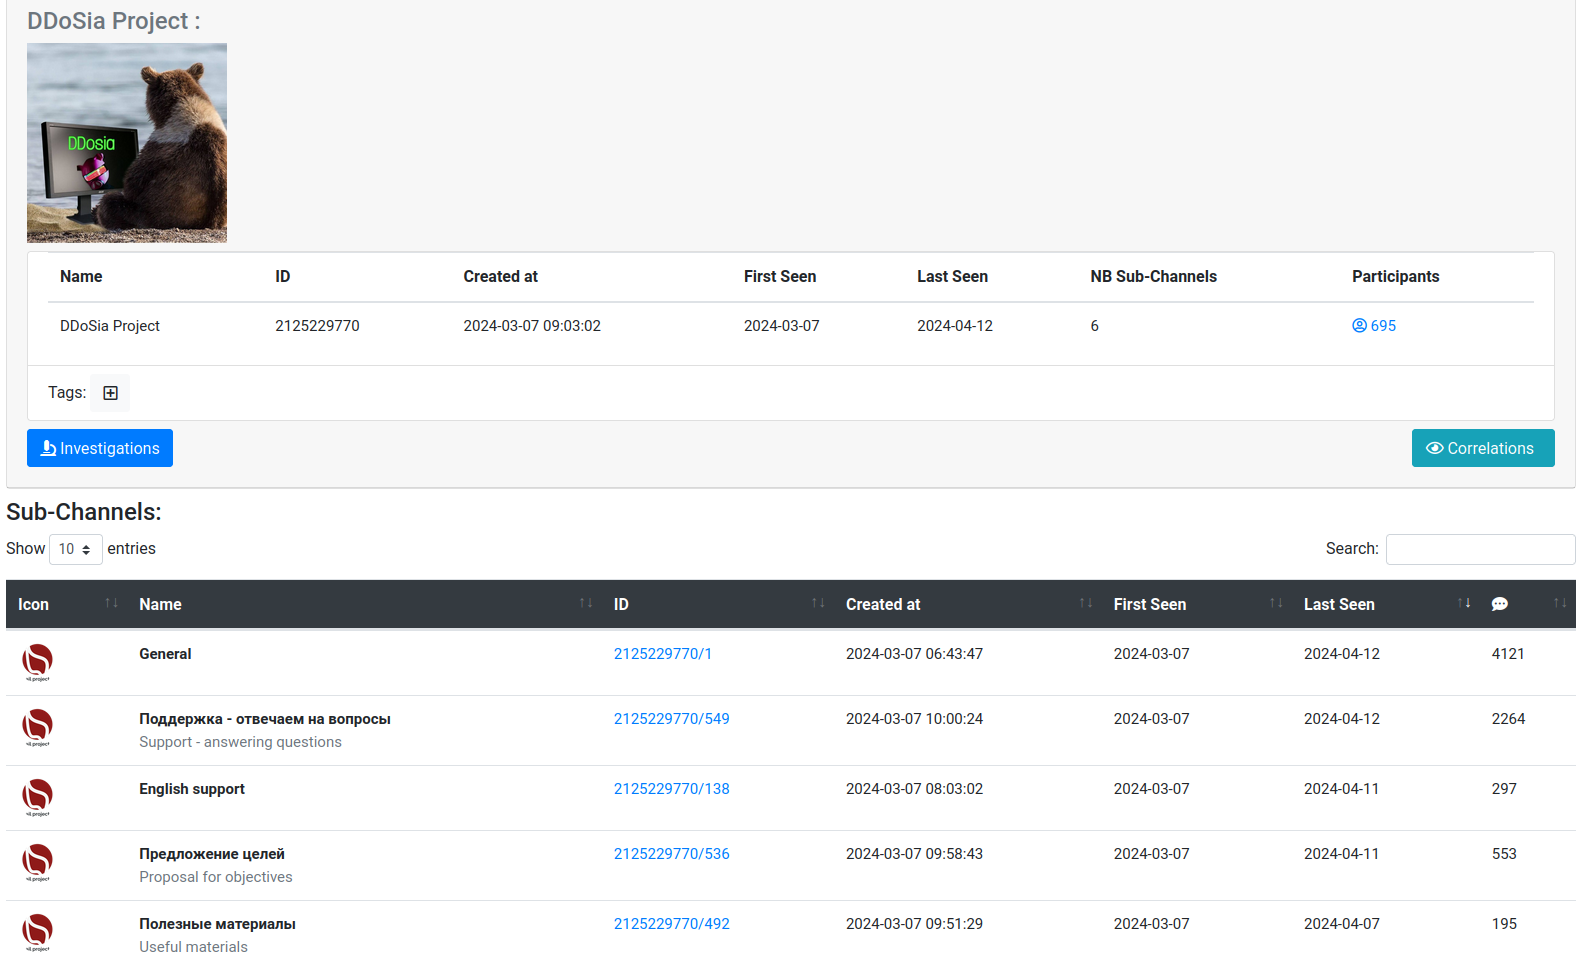
\includegraphics[scale=0.18]{screenshot/chat-forum.png}
\end{center}
\end{frame}

% TODO Processing ISSUES
%\begin{frame}
%    \frametitle{{\it Processing - Chats TODO GRAPH}}
%	\begin{itemize}
%		\item Processing automatically collected information can be a challenging task.
%		\item Chats image + description 
%		\item user image + description 
%		\item message + meta
%	\end{itemize}
%\end{frame}

\begin{frame}
    \frametitle{Processing - OCR - Next Release v5.5}
    \begin{center}
        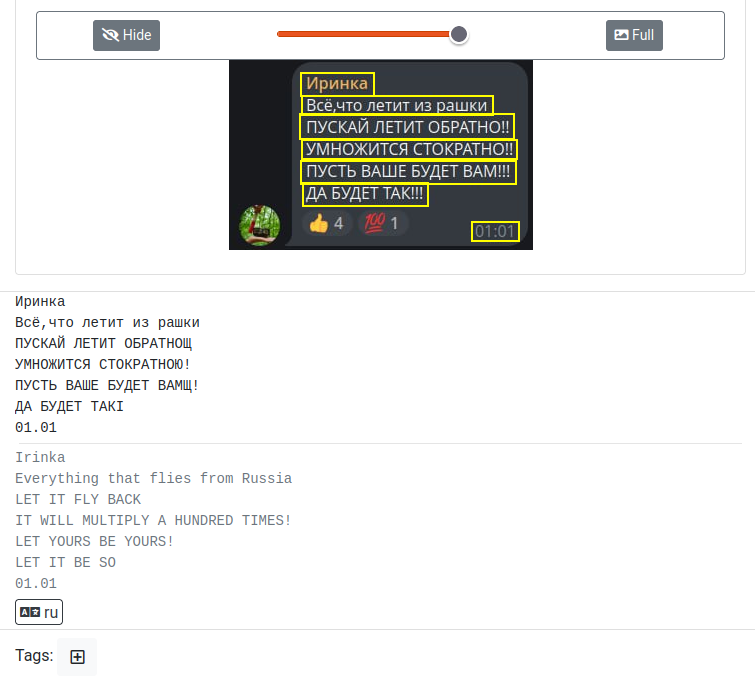
\includegraphics[scale=0.32]{screenshot/ail-ocr.png}
    \end{center}
\end{frame}

\begin{frame}
    \frametitle{Analysis of unstructured information}
    \begin{center}
        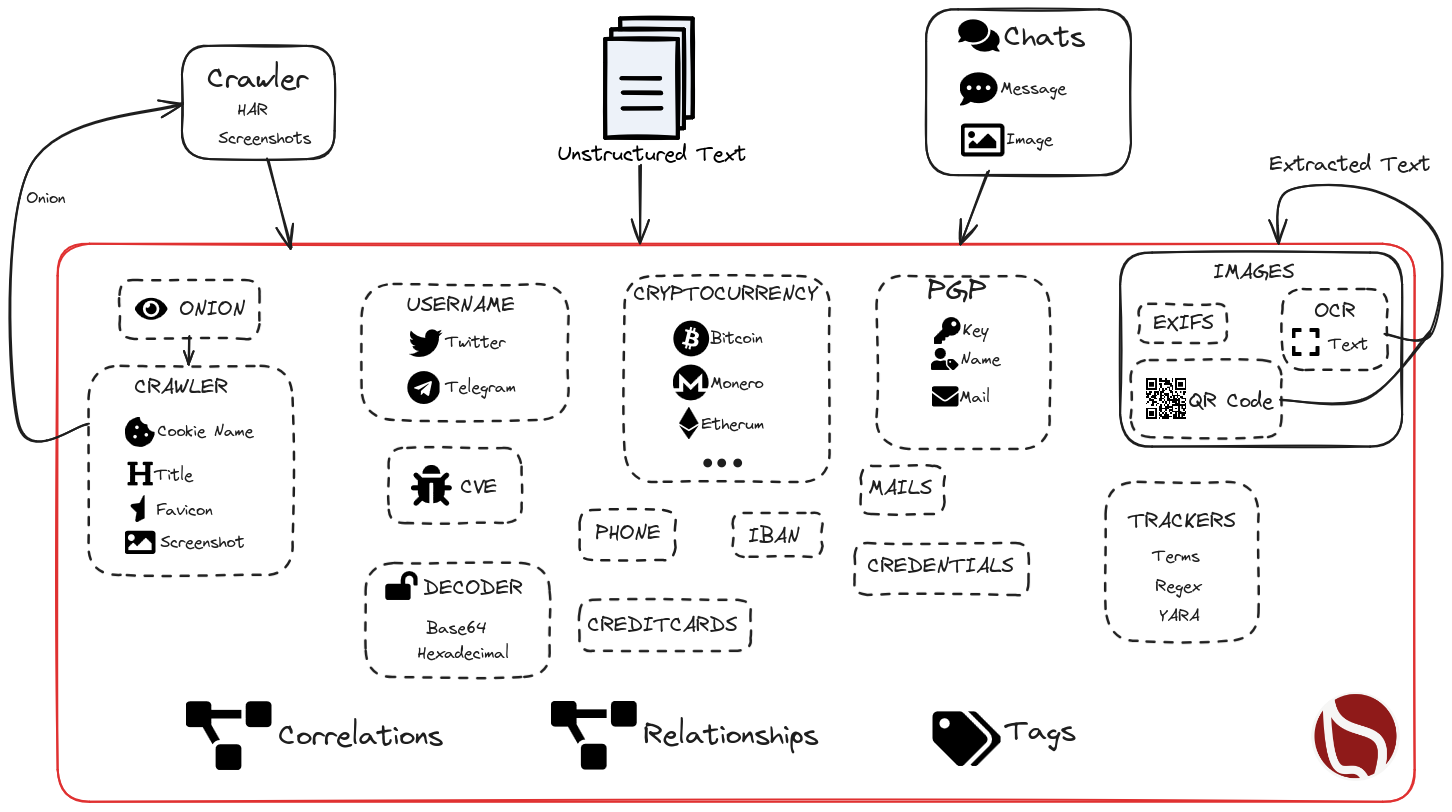
\includegraphics[scale=0.225]{images/ail-internal.png}
    \end{center}
\end{frame}

\begin{frame}
    \frametitle{AIL Framework: Current features}
    \begin{itemize}
        \item Extracting \textbf{credit cards numbers, credentials, phone numbers, ...}
        \item Extracting and validating potential \textbf{hostnames}
        \item Keeps track of \textbf{duplicates}
        \item Submission to threat sharing and incident response platform (\textbf{MISP} and \textbf{TheHive})
        \item \textbf{Full-text indexer} to index unstructured information
        \item \textbf{Tagging} for classification and searches
        \item Terms, sets, regex and YARA \textbf{tracking and occurrences}
        \item Archives, files and raw \textbf{submission} from the UI
        \item PGP, Cryptocurrency, Decoded (Base64, ...) and username Correlation
        \item And many more
    \end{itemize}
\end{frame}


\begin{frame}
    \frametitle{Trackers - Retro Hunt}
        \begin{itemize}
        	\item Search and monitor specific keywords/patterns
        	\begin{itemize}
            	\item Automatic Tagging
            	\item Email Notifications
            \end{itemize}
            \item Track Word
            \begin{itemize}
            	\item ddos
            \end{itemize}
            \item Track Set
            \begin{itemize}
            	\item booter,ddos,stresser;2
            \end{itemize}
            \item Track Regex
            \begin{itemize}
            	\item circl\textbackslash.lu
            \end{itemize}
            \item YARA rules
            	\begin{itemize}
            	\item https://github.com/ail-project/ail-yara-rules
            \end{itemize}
        \end{itemize}
\end{frame}

\section{Live Demo}

\begin{frame}
    \frametitle{YARA Tracker}
        \begin{figure}
            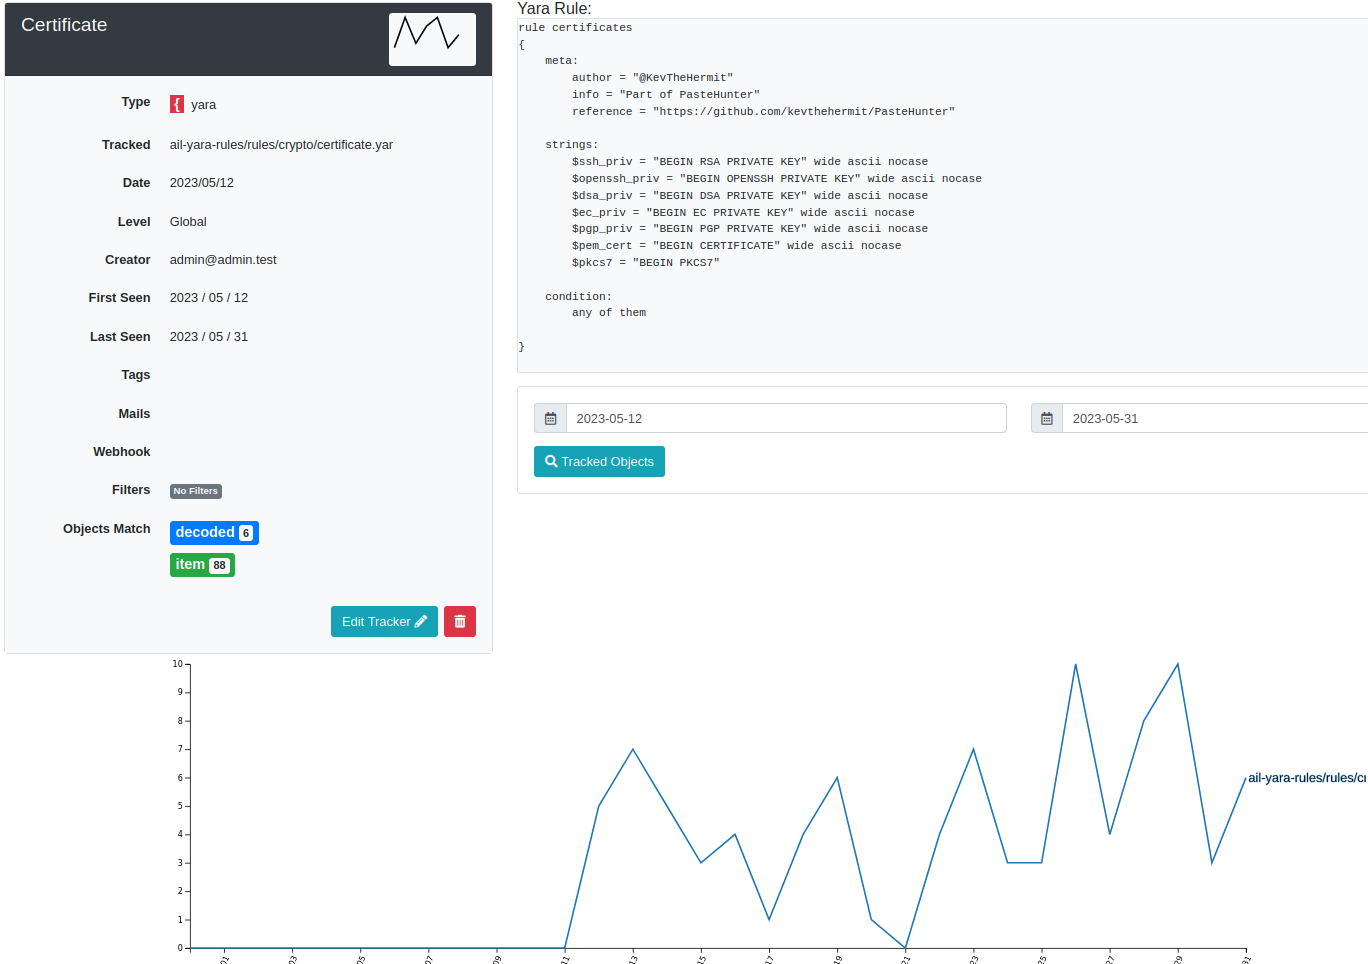
\includegraphics[scale=0.22]{screenshot/tracker_yara.png}
        \end{figure}
\end{frame}

\begin{frame}
    \frametitle{Retro Hunt}
        \begin{figure}
            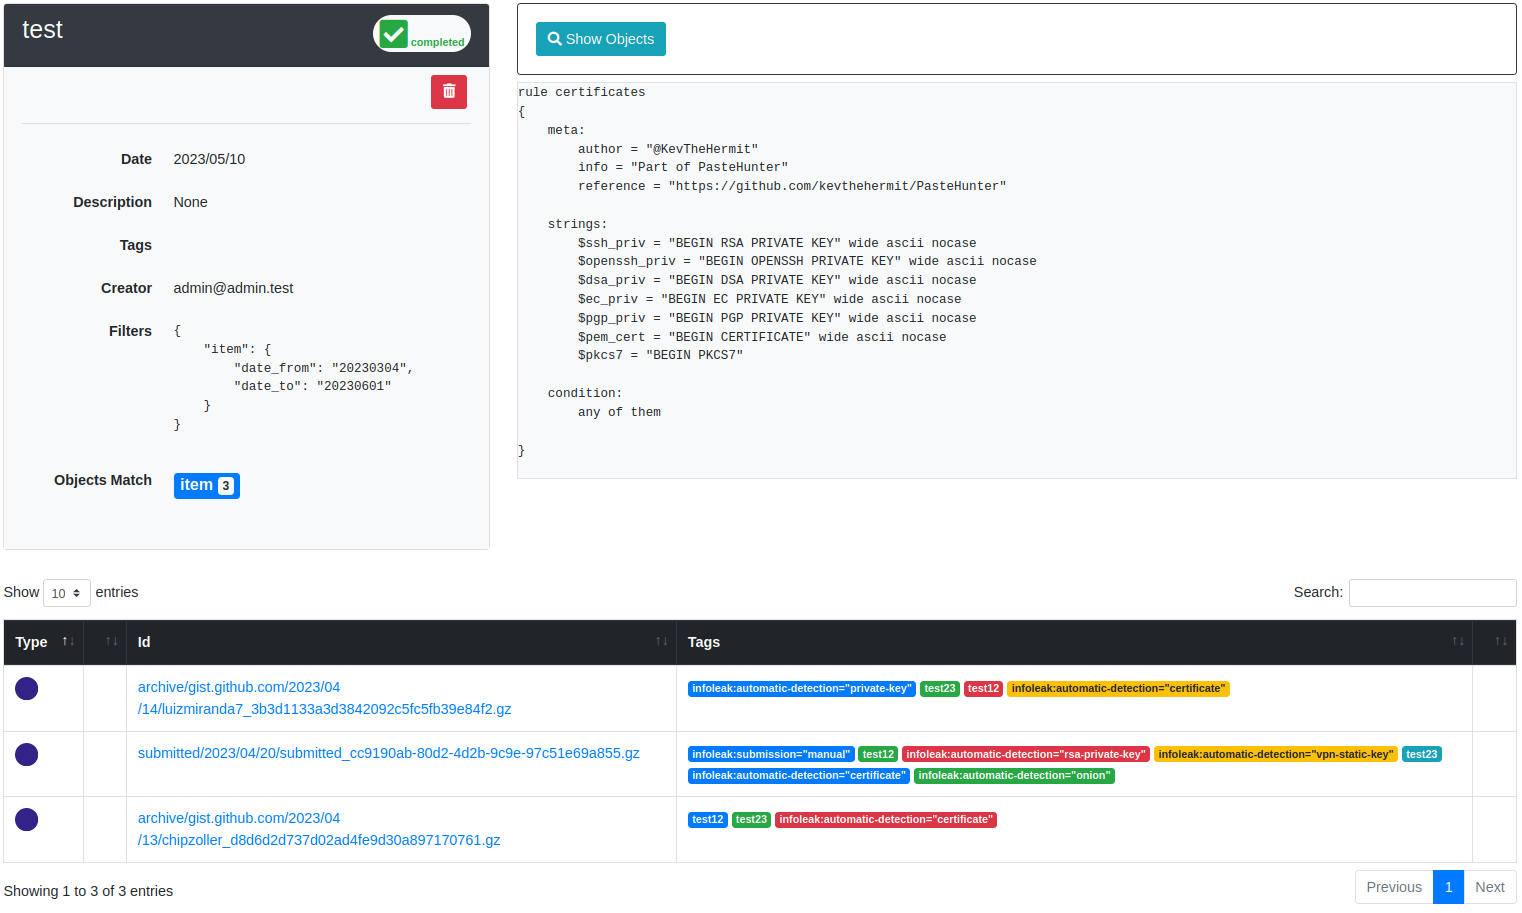
\includegraphics[scale=0.22]{screenshot/retro_hunt.png}
        \end{figure}
\end{frame}


\begin{frame}
    \frametitle{Correlations and relationship}
    \begin{figure}
        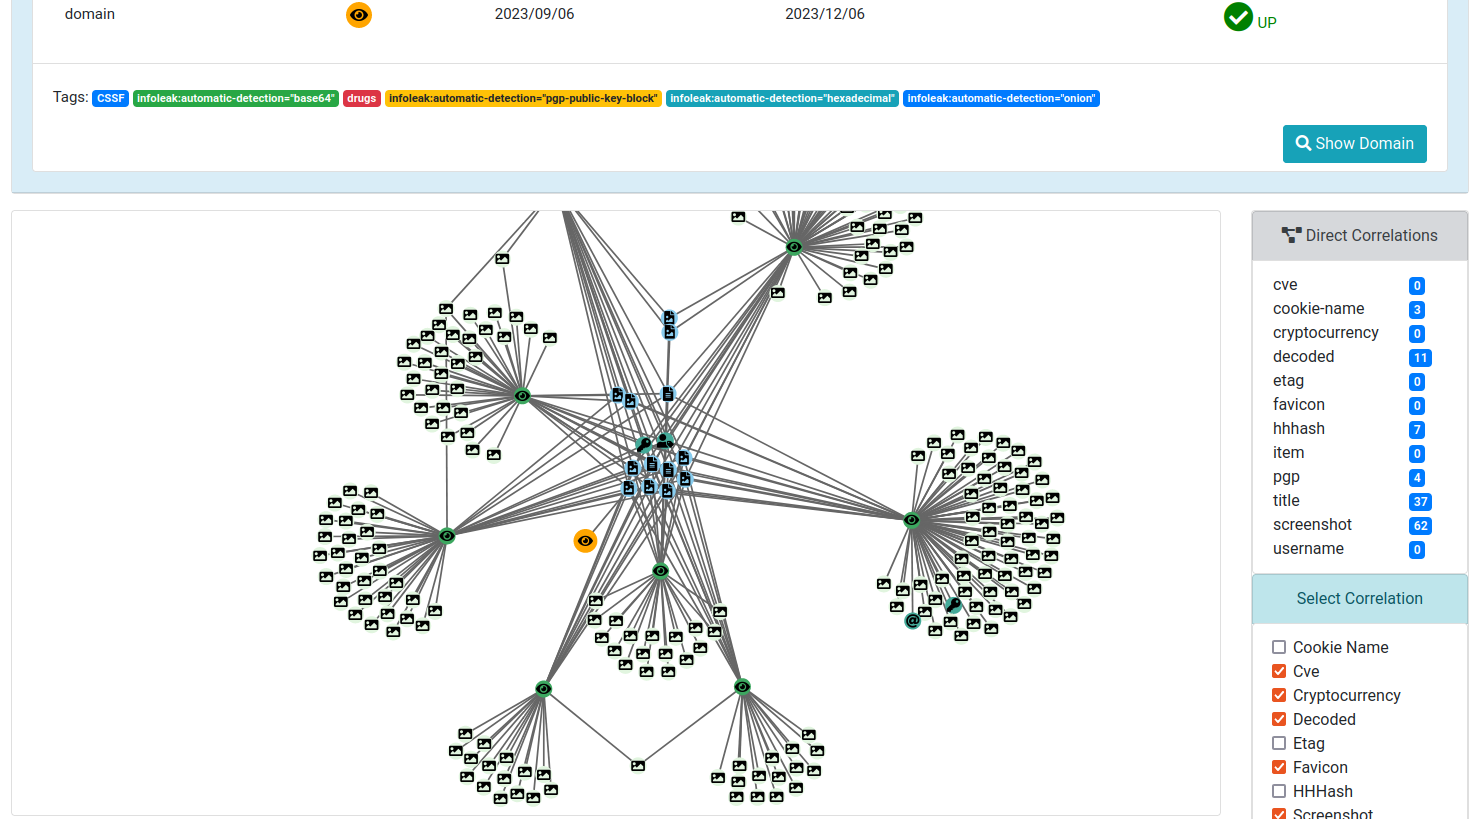
\includegraphics[scale=0.23, angle=0]{screenshot/ail-correlation.png}
    \end{figure}
\end{frame}


\begin{frame}
    \frametitle{Investigations}
    \begin{figure}
        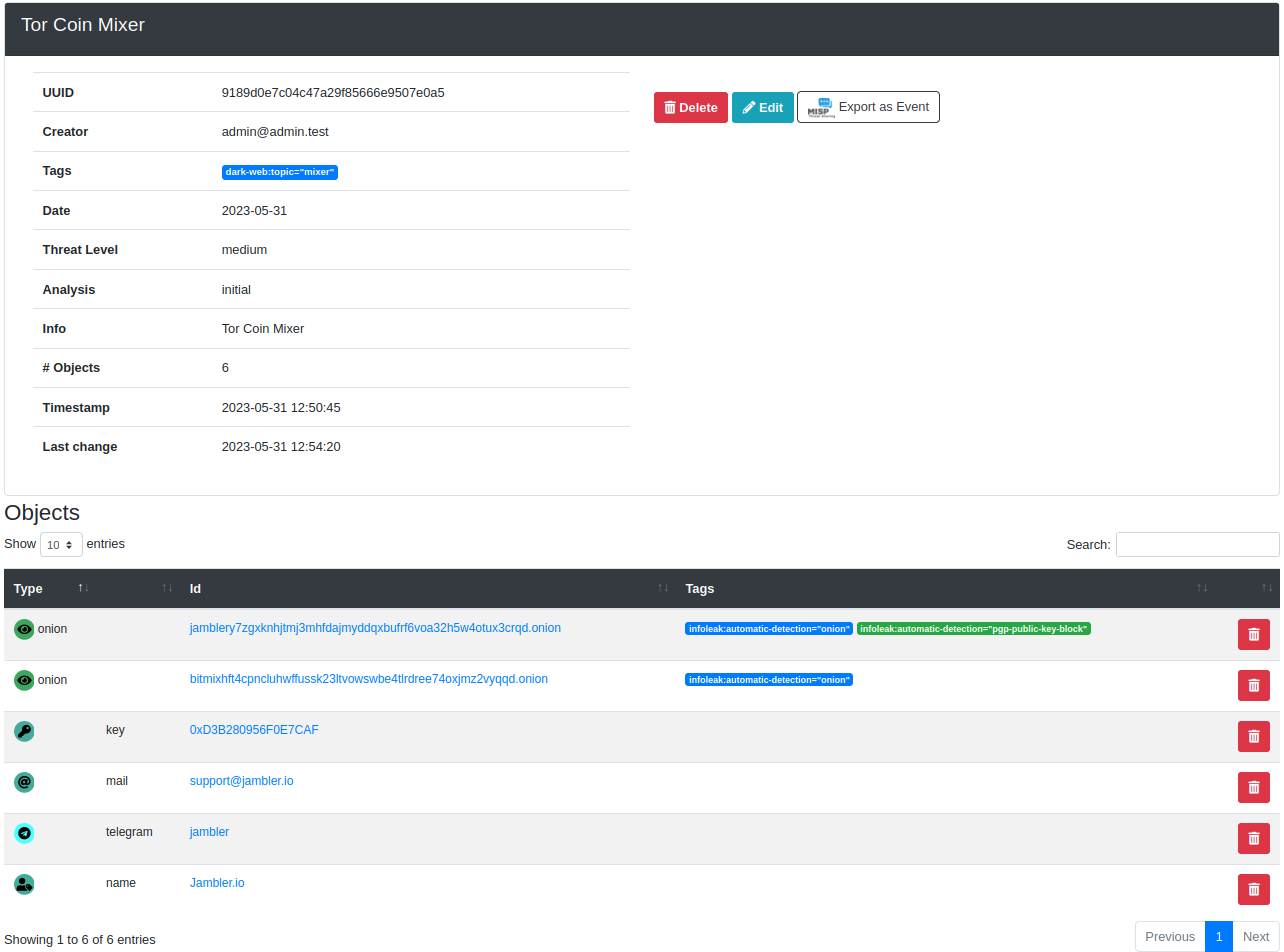
\includegraphics[scale=0.22, angle=0]{screenshot/investigation_mixer.png}
    \end{figure}
\end{frame}

\begin{frame}
    \frametitle{AIL Framework: Current capabilities}
    \begin{itemize}
        \item Extending AIL to add a new {\bf analysis module} can be done in 50 lines of Python
        \item The framework {\bf supports multi-processors/cores by default}. Any analysis module can be started multiple times to support faster processing during peak times or bulk import
        \item \textbf{Multiple} concurrent \textbf{data input}
        \item Tor Crawler (handle cookies authentication)
        \item Feeders: Discord, Telegram, ...
    \end{itemize}
\end{frame}


\begin{frame}
    \frametitle{{\bf MISP - LEA}}
		\begin{itemize}
    		\item Law enforcement agency information sharing community
    		\item AIL-LEA instance hosted by CIRCL
    		\item Request access by sending a mail to {\bf info@misp-lea.org} or {\bf info@circl.lu}
    		\item Request for free training {\bf info@misp-lea.org} or {\bf info@circl.lu}
		\end{itemize}
    	\begin{center}
        	
\includegraphics[scale=0.3]{images/misp-lea.png}
    	\end{center}
\end{frame}



\begin{frame}
	\frametitle{Ongoing developments}
        \begin{itemize}
			\item 2FA - OTP
            \item OCR extraction
			\item Bloom filter filtering - PSS
        	\item Relationships between Chats: message forwards, replies, ...
        \end{itemize}
\end{frame}


\begin{frame}
    \frametitle{Private Search Set (PSS)}
    \begin{center}
        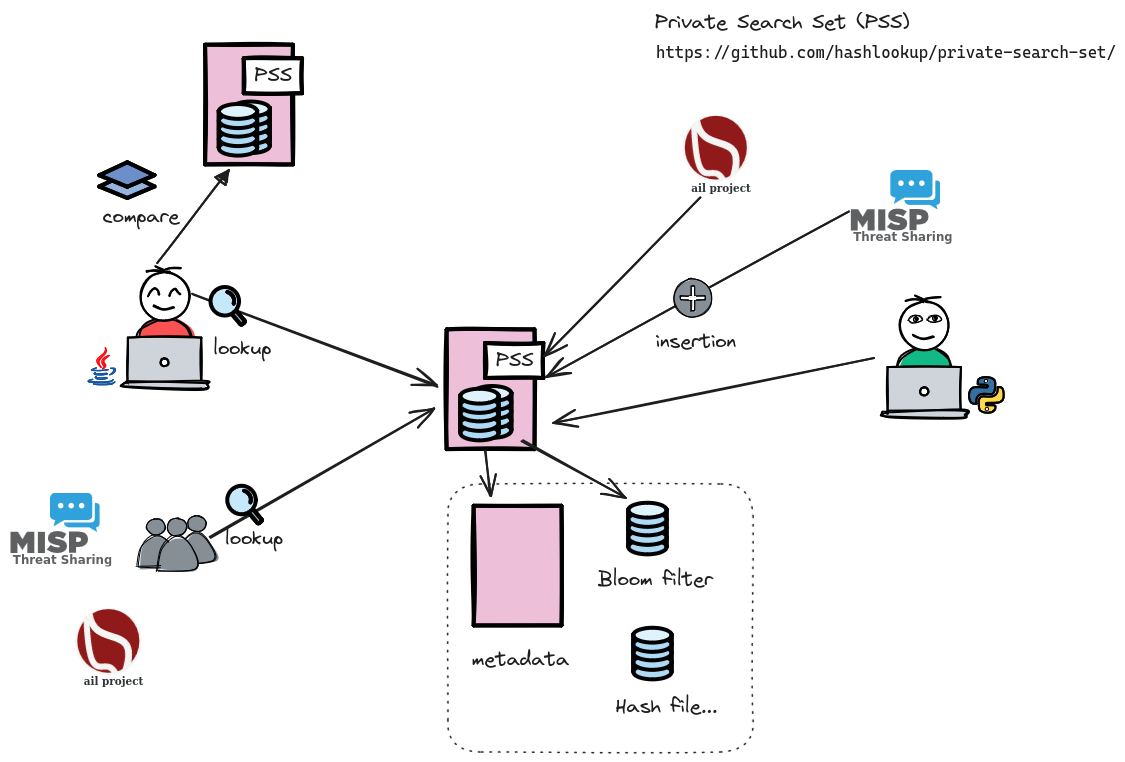
\includegraphics[scale=0.27]{images/pss-overview.png}
    \end{center}
\end{frame}


% LINKS
\begin{frame}
\frametitle{Links}
    \begin{itemize}
        \item AIL project \url{https://ail-project.org}
        \item Open Source \url{https://github.com/ail-project}
        \item Training materials  \url{https://github.com/ail-project/ail-training}
        \item Online chat \url{https://gitter.im/ail-project/community}
    \end{itemize}
    \begin{figure}
        
\includegraphics[scale=0.1, angle=0]{images/ail-project.png}
    \end{figure}
\end{frame}


\end{document}

